\documentclass[twoside,10pt]{article}
\usepackage{amsmath,amsfonts,amsthm,fullpage,amssymb}
%\usepackage{mymath}
%\usepackage{algorithm}
\usepackage{algorithmic}
\usepackage[]{algorithm2e}
\usepackage{graphicx}
\usepackage{url}
\usepackage{tcolorbox}
\usepackage{xcolor}
\usepackage{hyperref}


\begin{document}

\title{ISYE 6740 Homework 4\\ 
\small Total 100 points + 15 bonus points. }
\author{Shasha Liao}
\date{Deadline: Oct. 14, Wed., 11:59pm}
\maketitle

%----------------------------------------------------------------------------------
\begin{enumerate}

\item {\bf Basic optimization.} (40 points.)

Consider a simplified logistic regression problem. 
Given $m$ training samples $(x^i, y^i)$, $i = 1, \ldots, m$. The data $x^i \in \mathbb R$ (note that we only have one feature for each sample), and $y^i \in \{0, 1\}$.  To fit a logistic regression model for classification, we solve the following optimization problem, where $\theta \in \mathbb R$ is a parameter we aim to find:
\begin{equation}
\max_\theta \ell (\theta), \label{eqn}
\end{equation}
where the log-likelhood function \[\ell(\theta) = \sum_{i=1}^m \left\{-\log (1+\exp\{-\theta x^i\}) + (y^i-1) \theta x^i\right\}.\]

\begin{enumerate}
\item (10 points) Show step-by-step mathematical derivation for the gradient of the cost function $\ell(\theta)$ in (\ref{eqn}).
\begin{tcolorbox}
\textbf{Solution:} Since $\theta \in \mathbb R$, the gradient of $\ell(\theta)$ is just the derivative of $\ell(\theta)$. Then by Chain rule, we have
\begin{align*}
 \ell'(\theta) &= \sum_{i=1}^m \frac{d}{d \theta} \left\{ -\log (1+\exp\{-\theta x^i\})\right\} + \frac{d}{d \theta} \left\{ (y^i-1) \theta x^i\right\}\\
 &= \sum_{i=1}^m \left\{  -\frac{\frac{d}{d \theta} (1+\exp\{-\theta x^i\}) }{1+\exp\{-\theta x^i\}}+ \frac{d}{d \theta} \left\{ (y^i-1) \theta x^i\right\}\right\}\\
 &= \sum_{i=1}^m  \left\{ \frac{x^i\exp\{-\theta x^i\}} {1+\exp\{-\theta x^i\}} + (y^i-1)x^i\right\}.\\
\end{align*}
\end{tcolorbox}

\item (10 points) Write a pseudo-code  for performing {\bf gradient descent} to find the optimizer $\theta^*$. This is essentially what the training procedure does. (pseudo-code  means you will write down the steps of the algorithm, not necessarily any specific programming language.)
\begin{tcolorbox}
\textbf{Solution:} We may adjust the learning rate $\gamma$ base on the rate of convergence. \\
\begin{algorithm}[H]
\SetKwRepeat{Do}{do}{while}
 \KwData{$(x^i, y^i)$ for $i = 1, ..., m.$}
 \KwResult{${\theta^*}$}
 Initialization: $\theta^0, \gamma, \epsilon$\;
 \Do{$\|\theta^{t+1} - \theta^t\| > \epsilon$}{
  $\theta^{t+1} \leftarrow  \theta^t + \gamma \sum_{i=1}^m  \left\{ \frac{x^i\exp\{-\theta x^i\}} {1+\exp\{-\theta x^i\}} + (y^i-1)x^i\right\}$\;
 }
 \caption{Batch Gradient Descent}
\end{algorithm}
\end{tcolorbox}

\item (10 points) Write the pseudo-code for performing the {\bf stochastic gradient descent} algorithm to solve the training of logistic regression problem (\ref{eqn}). Please explain the difference between gradient descent and stochastic gradient descent for training logistic regression.
\begin{tcolorbox}
\textbf{Solution:} We may tune the learning rate $\gamma^0$ base on the rate of convergence. \\
\begin{algorithm}[H]
\SetKwRepeat{Do}{do}{while}
 \KwData{$(x^i, y^i)$ for $i = 1, ..., m.$}
 \KwResult{${\theta^*}$}
 Initialization: $\theta^0, \gamma^0, \epsilon, K$\;
 Randomly split the indices of our data points into subsets $S_k$, $k = 1, 2, ..., K$  \;
 
 
 \Do{ $\| \sum_{i=1}^m  \left\{ \frac{x^i\exp\{-\theta x^i\}} {1+\exp\{-\theta x^i\}} + (y^i-1)x^i \right\} \| > \epsilon$}
  {
      \For{$k = 1, 2, ..., K$}
          {
                $\theta^{t+1} \leftarrow  \theta^t + \gamma^t \sum_{i \in S_k}  \left\{ \frac{x^i\exp\{-\theta x^i\}} {1+\exp\{-\theta x^i\}} + (y^i-1)x^i\right\}$\;
                $\gamma^{t+1} \leftarrow \frac{\gamma^0}{t+1}$          
          }
  }
 
 \caption{Stochastic Gradient Descent}
\end{algorithm}
\break
Comparing GD(Gradient Descent) and SGD(Stochastic Gradient Descent):
\begin{itemize}
\item Way of Convergence: GD increases the likelihood function value at each iteration as long as we choose a suitable learning rate,  while SGD may not increase the likelihood function value at each step but will decrease it in an oscillating fashion.
\item Speed of Convergence: For a large dataset, GD converges very slowly since it utilize all the data for one single update of $\theta$, while SGD can converge much faster as it only utilize a small subset of the data for each update of $\theta$.
\item Conclusion: If the data set is small, I prefer GD as the computation can still be fast and it increase the likelihood  at each step. If the data set is large, I prefer SGD for a faster rate of convergence.
\end{itemize}
\end{tcolorbox}

\item (10 points) We will {\bf show that the training problem in basic logistic regression problem is concave.} Derive the Hessian matrix of $\ell(\theta)$ and based on this, show the training problem (\ref{eqn}) is concave (note that in this case, since we only have one feature, the Hessian matrix is just a scalar). Explain why the problem can be solved efficiently and gradient descent will achieve a unique global optimizer, as we discussed in class. 
\begin{tcolorbox}
\textbf{Solution:} From part (a), we have
\begin{align*}
 \ell'(\theta)  &= \sum_{i=1}^m  \left\{ \frac{x^i\exp\{-\theta x^i\}} {1+\exp\{-\theta x^i\}} + (y^i-1)x^i\right\}.\\
\end{align*}
\end{tcolorbox}

\begin{tcolorbox}
So
\begin{align*}
 \ell''(\theta)  &= \sum_{i=1}^m \frac{d}{d\theta}  \left\{ \frac{x^i\exp\{-\theta x^i\}} {1+\exp\{-\theta x^i\}} + (y^i-1)x^i\right\}\\
 &= \sum_{i=1}^m \frac{d}{d\theta} \frac{-x^i} {1+\exp\{-\theta x^i\}} \\
 &=  \sum_{i=1}^m  \frac{-(x^i)^2} {(1+\exp\{-\theta x^i\})^2} \\
 &<0.
\end{align*}
Therefore, $\ell(\theta)$ is a concave function and has a unique global maximum point.
\end{tcolorbox}

\end{enumerate}
 
\item {\bf Comparing Bayes, logistic, and KNN classifiers.} (60 points)

In lectures, we learn three different classifiers. This question is to implement and compare them. Python users, please feel free to use \textsf{Scikit-learn}, which is a commonly-used and powerful \textsf{Python} library with various machine learning tools. But you can also use other similar libraries in other languages of your choice to perform the tasks. 


\textbf{Part One (Divorce classification/prediction).} (30 points) 

This dataset is about participants who completed the personal information form and a divorce predictors scale. 

The data is a modified version of the publicly available at \\ \url{https://archive.ics.uci.edu/ml/datasets/Divorce+Predictors+data+set} (by injecting noise so you will not get the exactly same results as on UCI website).  The dataset \textbf{marriage.csv} is contained in the homework folder. There are 170 participants and 54 attributes (or predictor variables) that are all real-valued. The last column of the CSV file is label $y$ (1 means ``divorce'', 0 means ``no divorce''). Each column is for one feature (predictor variable), and each row is a sample (participant). A detailed explanation for each feature (predictor variable) can be found at the website link above. Our goal is to build a classifier using training data, such that given a test sample, we can classify (or essentially predict) whether its label is 0 (``no divorce'') or 1 (``divorce''). 

Build three classifiers using ({\bf Naive Bayes, Logistic Regression, KNN}). Use the first $80\%$ data for training and the remaining $20\%$ for testing. If you use \textsf{scikit-learn} you can use \textsf{train\_test\_split} to split the dataset. 

\textit{Remark: Please note that, here, for Naive Bayes, this means that we have to estimate the variance for each individual feature from training data. When estimating the variance, if the variance is zero to close to zero (meaning that there is very little variability in the feature), you can set the variance to be a small number, e.g., $\epsilon = 10^{-3}$. We do not want to have include zero or nearly variance in Naive Bayes. This tip holds for both Part One and Part Two of this question.}

\textit{{\color{red} If we have a feature $x_i$ with constant value, then Naive Bayes will suffer from dividing by zero when it tries to fit a Gaussian distribution for $x_i$ since the variance of $x_i$ is zero. In Sklearn GaussianNB, this issue is avoided by using a parameter \textbf{var\_smoothing}, which is the portion of the largest variance of all features that is added to variances for calculation stability. If \textbf{var\_smoothing} is too large, the fitted Naive Bayes model will suffer from under-fitting because large variances lead to a simple model.  }}

\begin{enumerate}

	\item (15 points) Report testing accuracy for each of the three classifiers.  Comment on their performance: which performs the best and make a guess why they perform the best in this setting. 
	\begin{tcolorbox}
	\textbf{Solution:} \\
	\begin{center}
	\begin{tabular}{| c | c |}%??c?????????????(center)
	\hline
	Classifier & Testing accuracy \\
	\hline
        Naive Bayes & 1.00 \\%??????????  ???&??
        \hline
        Logistic Regression &0.85\\%??????????  ???&??
        \hline
        KNN & 1.00\\
        \hline
        \end{tabular}
        \end{center}
        From the table above, we see that Naive Bayes and KNN did a much better job than Logistic Regression. I guess the reason is that the two classes in the testing set are not linear separable in the 54 dimensional feature space, which explains that the nonlinear classifiers like Naive Bayes and KNN perform better than the linear classifier Logistic Regression.
	\end{tcolorbox}
	\item (15 points) Now perform PCA to project the data into two-dimensional space. Plot the data points and decision boundary of each classifier. Comment on the difference between the decision boundary for the three classifiers. Please clearly represent the data points with different labels using different colors.
\begin{tcolorbox}
\textbf{Solution:}\\

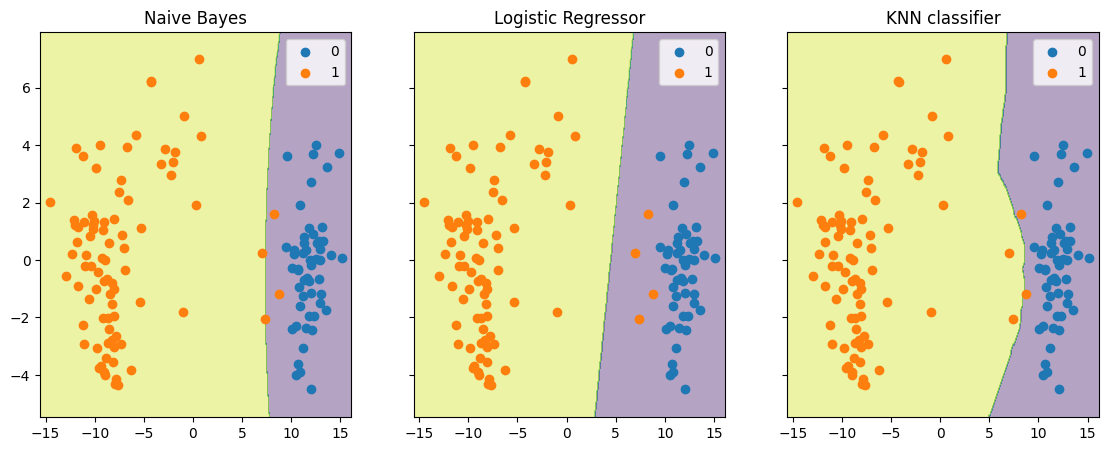
\includegraphics[width=\linewidth]{divorce.png}
Clearly, Logistic Regressor has a perfect linear decision boundary, while both Naive Bayes and KNN has nonlinear decision boundaries. 


\end{tcolorbox}
	
\end{enumerate}

\textbf{Part Two (Handwritten digits classification).} (30 points) Repeat the above using the \textbf{MNIST Data} in our previous homework. Here, give ``digit'' 6 label $y = 1$, and give ``digit'' 2 label $y = 0$. All the pixels in each image will be the feature (predictor variables) for that sample (i.e., image). Our goal is to build classifier to such that given a new test sample, we can tell is it a 2 or a 6. Using the first $80\%$ of the samples for training and remaining $20\%$ for testing. 
\begin{enumerate}
\item (15 points) Report testing accuracy for each of the three classifiers.  Comment on their performance: which performs the best and make a guess why they perform the best in this setting. 
\begin{tcolorbox}
\textbf{Solution:}\\
\begin{center}
	\begin{tabular}{| c | c |}%??c?????????????(center)
	\hline
	Classifier & Testing accuracy \\
	\hline
        Naive Bayes & 0.97 \\%??????????  ???&??
        \hline
        Logistic Regression &0.96\\%??????????  ???&??
        \hline
        KNN & 1.00\\
        \hline
        \end{tabular}
        \end{center}
KNN has the highest accuracy this time. This might due to the highly nonlinearity of the actual boundary between the two classes in testing set. Even though Naive Bayes also has nonlinear boundaries, it is restricted to piecewise quadratic decision boundaries. So, Naive Bayes is not as flexible as KNN. The results shows that the more nonlinearity a decision boundary has, the higher accuracy it achieves. 
\end{tcolorbox}

	\item (15 points) Now perform PCA to project the data into two-dimensional space. Plot the data points and decision boundary of each classifier. Comment on the difference between the decision boundary for the three classifiers. Please clearly represent the data points with different labels using different colors.
\begin{tcolorbox}
\textbf{Solution:}\\
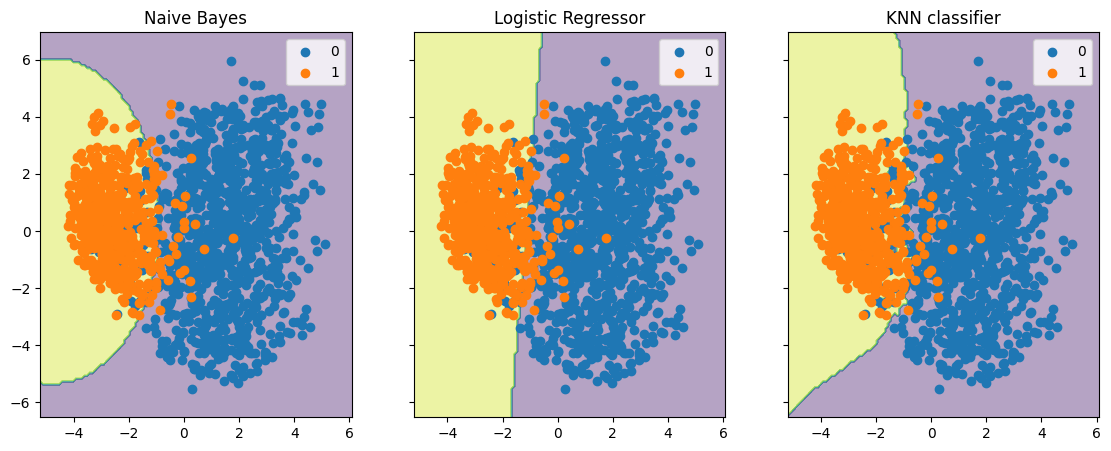
\includegraphics[width=\linewidth]{MNIST.png}
Naive Bayes has a piecewise quadratic decision boundary. Logistic Regressor has a linear decision boundary. KNN has a highly nonlinear decision boundary. 
\end{tcolorbox}
\end{enumerate}

\item {\bf Naive Bayes for spam filtering}. (15 points) %(Bonus question: 20 points) 

In this problem, we will use the Naive Bayes algorithm to fit a spam filter by hand. This will enhance your understanding to Bayes classifier and build intuition. This question does not involve any programming but only derivation and hand calculation. 

Spam filters are used in all email services to classify received emails as ``Spam'' or ``Not Spam''. A simple approach involves maintaining a vocabulary of words that commonly occur in ``Spam'' emails and classifying an email as ``Spam'' if the number of words from the dictionary that are present in the email is over a certain threshold.
We are given the vocabulary consists of 15 words \[V=\{\textsf{secret, offer, low, price, valued, customer, today, dollar, million, sports, is, for, play, healthy, pizza}\}.\] We will use $V_i$ to represent the $i$th word in $V$. As our training dataset, we are also given 3 example spam messages,
\begin{itemize}
\item \textsf{million dollar offer}
\item \textsf{secret offer today}
\item \textsf{secret is secret}
\end{itemize}
and 4 example non-spam messages
\begin{itemize}
\item \textsf{low price for valued customer}
\item \textsf{play secret sports today}
\item \textsf{sports is healthy}
\item \textsf{low price pizza}
\end{itemize}

Recall that the Naive Bayes classifier assumes the probability of an input depends on its input feature. The feature for each sample is defined as
$x^{(i)} = [x_1^{(i)}, x_2^{(i)}, \ldots, x_d^{(i)}]^T$, $i = 1, \ldots, m$ and the class of the $i$th sample is $y^{(i)}$. In our case the length of the input vector is $d = 15$, which is equal to the number of words in the vocabulary $V$. Each entry $x_j^{(i)}$ is equal to the number of times word $V_j$ occurs in the $i$-th message. %The marginal distribution of 

\begin{enumerate}
\item (5 points) Calculate class prior $\mathbb P(y = 0)$ and $\mathbb P(y = 1)$ from the training data, where $y = 0$ corresponds to spam messages, and $y = 1$ corresponds to non-spam messages. Note that these class prior essentially corresponds to the frequency of each class in the training sample. Write down the feature vectors for each spam and non-spam messages.
\begin{tcolorbox}
\textbf{Solution:} $\mathbb P(y = 0) = \frac 3 7$ and $\mathbb P(y = 1) = \frac 4 7$.
\begin{center}
	\begin{tabular}{| c | c | c |}%??c?????????????(center)
	\hline
& Messages & Feature vectors \\
\hline
& million dollar offer & [0, 1, 0, 0, 0, 0, 0, 1, 1, 0, 0, 0, 0, 0, 0] \\
Spam & secret offer today & [1, 1, 0, 0, 0, 0, 1, 0, 0, 0, 0, 0, 0, 0, 0] \\
& secret is secret & [2, 0, 0, 0, 0, 0, 0, 0, 0, 0, 1, 0, 0, 0, 0] \\
\hline
& low price for valued customer & [0, 0, 1, 1, 1, 1, 0, 0, 0, 0, 0, 1, 0, 0, 0] \\
Non-spam & play secret sports today & [1, 0, 0, 0, 0, 0, 1, 0, 0, 1, 0, 0, 1, 0, 0] \\
& sports is healthy & [0, 0, 0, 0, 0, 0, 0, 0, 0, 1, 1, 0, 0, 1, 0] \\
& low price pizza & [0, 0, 1, 1, 0, 0, 0, 0, 0, 0, 0, 0, 0, 0, 1] \\
 \hline
        \end{tabular}
        \end{center}
\end{tcolorbox}

\item (5 points) In the Naive Bayes model, assuming the keywords are independent of each other (this is a simplification), the likelihood of a sentence with its feature vector $x$ given a class $c$ is given by 
\[
\mathbb P (x|y = c) = \prod_{k=1}^d \theta_{c, k}^{x_k}, \quad c = \{0, 1\}
\]
where $0 \leq \theta_{c,k} \leq 1$ is the probability of word $k$ appearing in class $c$, which satisfies 
\[\theta_{0,k} = 1- \theta_{1, k} , \quad \forall k.\] Given this, the complete log-likelihood function for our training data is given by
\[
\ell(\theta_{0,1}, \ldots, \theta_{0, d}, \theta_{1,1}, \ldots, \theta_{1, d}) = 
\sum_{i=1}^m \sum_{k=1}^d x_k^{(i)} \log \theta_{y^{(i)}, k}
\]
(In this example, $m = 7$.)
 Calculate the maximum likelihood estimates of $\theta_{0,1}$, $\theta_{0,7}$, $\theta_{1,1}$, $\theta_{1,15}$ by maximizing the log-likelihood function above.
 %$\mathbb P (x|y = c)$ with respect to $\theta_{c, k}$ and given data. 
 (Hint: We are solving a constrained maximization problem: you can introduce Lagrangian multipliers, or directly substitute the $\theta_{0,k} = 1- \theta_{1, k}$ into the objective function so you do not need to worry about the constraint.)
\begin{tcolorbox}
\textbf{Solution:}\\
$ i =  1  : x^{(1)}_{2} = 1, x^{(1)}_{8} = 1, x^{(1)}_{9} = 1, $\\

$ i =  2  : x^{(2)}_{1} = 1, x^{(2)}_{2} = 1, x^{(2)}_{7} = 1, $\\

$ i =  3  : x^{(3)}_{1} = 2, x^{(3)}_{11} = 1, $\\

$ i =  4  : x^{(4)}_{3} = 1, x^{(4)}_{4} = 1, x^{(4)}_{5} = 1, x^{(4)}_{6} = 1, x^{(4)}_{12} = 1, $\\

$ i =  5  : x^{(5)}_{1} = 1, x^{(5)}_{7} = 1, x^{(5)}_{10} = 1, x^{(5)}_{13} = 1, $\\

$ i =  6  : x^{(6)}_{10} = 1, x^{(6)}_{11} = 1, x^{(6)}_{14} = 1, $\\

$ i =  7  : x^{(7)}_{3} = 1, x^{(7)}_{4} = 1, x^{(7)}_{15} = 1, $\\

\begin{align*}
\ell(\theta_{0,1}, \ldots, \theta_{0, d}, \theta_{1,1}, \ldots, \theta_{1, d}) & = \sum_{i=1}^m \sum_{k=1}^d x_k^{(i)} \log \theta_{y^{(i)}, k} \\
& = \sum_{k=1}^d ( \sum_{i=1}^3 x_k^{(i)} \log \theta_{0,k} + \sum_{i= 4}^7 x_{k}^{(i)} \log (1-\theta_{0,k}) ).\\
\end{align*}
From the equation above we see that maximizing $\ell$ is equivalent to maximizing $\sum_{i=1}^3 x_k^{(i)} \log \theta_{0,k} + \sum_{i= 4}^7 x_{k}^{(i)} \log (1-\theta_{0,k})$ for each $k$ separably, which can be reduced to solving the following optimization problem 
$$\max_{\theta \in [0,1]} a \log \theta + b \log (1- \theta), \quad a \geq 0, b\geq 0$$
where we define $\log 0 = -\infty$.
Denote $$f(\theta) = a \log \theta + b \log (1- \theta),$$ then $$ f'(\theta) = \frac a \theta - \frac b {1-\theta} = \frac{a - (a+b)\theta}{\theta(1-\theta)}. $$ To find the maximizer $\theta^*$, we just need to solve $f'(\theta^*) = 0$, we obtain $$\theta^* = \frac{a}{a+b}.$$
Therefore, for each $k$, we have $\theta_{0,k}^* = \frac{\sum_{i=1}^3 x^{(i)}_k}{\sum_{i=1}^7 x^{(i)}_k}$. So, 
\begin{align*}
\theta_{0,1}^* &= \frac 3 4,\\
\theta_{0,7}^* &= \frac 1 2,\\
\theta_{1,1}^* &= 1-  \theta_{0,1}^*  = 1- \frac 3 4 = \frac 1 4,\\
\theta_{1,15}^* &= 1-  \theta_{0,15}^*  = 1 -  0 = 1.\\
\end{align*}
\end{tcolorbox}

\item (5 points) Given a test message ``\textsf{today is secret}'', using the Naive Bayes classier that you have trained in Part (a)-(b), to calculate the posterior and decide whether it is spam or not spam.
\begin{tcolorbox}
\textbf{Solution:}\\
The vector for ``\textsf{today is secret}'' is $x$ with $x_1= 1, x_7=1,x_{11}= 1$ and all other components zero. 
Recall that $ \theta_{0,1}^* = \frac 3 4, \theta_{0,7}^* = \frac 1 2, \theta^*_{0,11} = \frac 1 2. $
\begin{itemize}
\item Evaluate the likelihoods:\\
$$\mathbb P(x|y=0) = \Pi _{k=1}^d (\theta^*_{0,k})^{x_k} = \theta^*_{0,1} \theta^*_{0,7} \theta^*_{0,11} = \frac 3 {16}.$$
$$\mathbb P(x|y=1) = \Pi _{k=1}^d (\theta^*_{1,k})^{x_k} = \theta^*_{1,1} \theta^*_{1,7} \theta^*_{1,11} = \frac 1 {16}.$$
\item Evaluate the prior probability: \\
$$\mathbb P(y = 0) = \frac 3 7.$$ $$\mathbb P(y = 1) = \frac 4 7.$$
\item Evaluate the posterior by Bayes Formula: \\

\begin{align*}
\mathbb P (y = 0 | x) &= \frac{\mathbb P (x| y = 0) \mathbb P(y=0)}{ \mathbb P (x| y = 0) \mathbb P(y=0) + \mathbb P (x| y = 1) \mathbb P(y=1) }\\
&= \frac{\frac{3}{16} \cdot \frac{3}{7}}{ \frac{3}{16} \cdot \frac{3}{7} + \frac{1}{16} \cdot \frac{4}{7} } \\
&= \frac{9}{13} > \frac 1 2.
\end{align*}
\end{itemize}
Since $\mathbb P (y = 0 | x) > \frac 1 2$, we classify the message ``\textsf{today is secret}'' as spam.
\end{tcolorbox}
\end{enumerate}

\end{enumerate}


\end{document}
